% Generated by code/needham.py -- do not edit by hand.
\definecolor{qocA}{rgb}{0.00,0.45,0.70}
\definecolor{qocB}{rgb}{0.90,0.60,0.00}
\definecolor{qocC}{rgb}{0.00,0.62,0.45}
\definecolor{qocD}{rgb}{0.80,0.40,0.00}
\definecolor{qocE}{rgb}{0.80,0.60,0.70}
\definecolor{qocF}{rgb}{0.35,0.70,0.90}
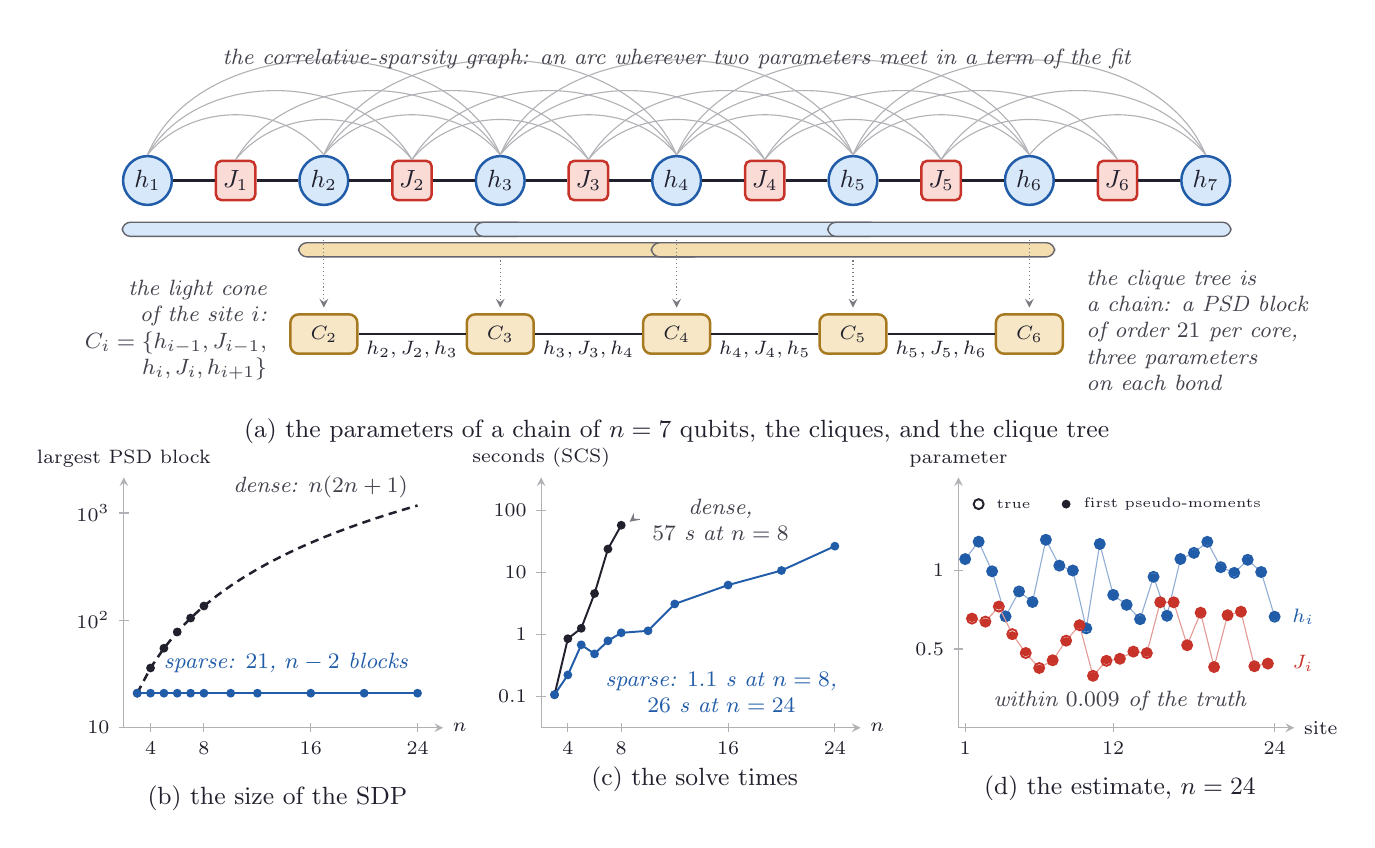
\begin{tikzpicture}[ink/.style={line width=0.9pt, ndInk}, faint/.style={line width=0.4pt, ndInk!35}, dashedink/.style={line width=0.5pt, ndInk!55, dash pattern=on 2.5pt off 2pt}, vec/.style={->, >=stealth, line width=1.2pt}, note/.style={font=\footnotesize\itshape, text=ndInk!85, align=center}, pointer/.style={->, >=stealth, line width=0.4pt, ndInk!60, shorten >=2pt, shorten <=1pt}, dot/.style={circle, fill=ndInk, inner sep=0pt, minimum size=3.4pt}, wash/.style={fill=ndSky, fill opacity=0.55}, every node/.style={text=ndInk}]
\definecolor{ndInk}{rgb}{0.13,0.13,0.18}
\definecolor{ndPaper}{rgb}{0.99,0.96,0.88}
\definecolor{ndSky}{rgb}{0.84,0.91,0.98}
\definecolor{ndRose}{rgb}{0.98,0.86,0.84}
\definecolor{ndBlue}{rgb}{0.13,0.36,0.66}
\definecolor{ndRed}{rgb}{0.78,0.20,0.16}
\definecolor{ndGold}{rgb}{0.88,0.62,0.10}
\definecolor{ndGreen}{rgb}{0.18,0.52,0.30}
\node[circle, draw=ndBlue, fill=ndSky, line width=0.9pt, minimum size=0.62cm, inner sep=0pt, font=\small] (v0) at (0.900,6.950) {$h_{1}$};
\node[rounded corners=2pt, draw=ndRed, fill=ndRose, line width=0.9pt, minimum size=0.5cm, inner sep=1pt, font=\small] (v1) at (2.020,6.950) {$J_{1}$};
\node[circle, draw=ndBlue, fill=ndSky, line width=0.9pt, minimum size=0.62cm, inner sep=0pt, font=\small] (v2) at (3.140,6.950) {$h_{2}$};
\node[rounded corners=2pt, draw=ndRed, fill=ndRose, line width=0.9pt, minimum size=0.5cm, inner sep=1pt, font=\small] (v3) at (4.260,6.950) {$J_{2}$};
\node[circle, draw=ndBlue, fill=ndSky, line width=0.9pt, minimum size=0.62cm, inner sep=0pt, font=\small] (v4) at (5.380,6.950) {$h_{3}$};
\node[rounded corners=2pt, draw=ndRed, fill=ndRose, line width=0.9pt, minimum size=0.5cm, inner sep=1pt, font=\small] (v5) at (6.500,6.950) {$J_{3}$};
\node[circle, draw=ndBlue, fill=ndSky, line width=0.9pt, minimum size=0.62cm, inner sep=0pt, font=\small] (v6) at (7.620,6.950) {$h_{4}$};
\node[rounded corners=2pt, draw=ndRed, fill=ndRose, line width=0.9pt, minimum size=0.5cm, inner sep=1pt, font=\small] (v7) at (8.740,6.950) {$J_{4}$};
\node[circle, draw=ndBlue, fill=ndSky, line width=0.9pt, minimum size=0.62cm, inner sep=0pt, font=\small] (v8) at (9.860,6.950) {$h_{5}$};
\node[rounded corners=2pt, draw=ndRed, fill=ndRose, line width=0.9pt, minimum size=0.5cm, inner sep=1pt, font=\small] (v9) at (10.980,6.950) {$J_{5}$};
\node[circle, draw=ndBlue, fill=ndSky, line width=0.9pt, minimum size=0.62cm, inner sep=0pt, font=\small] (v10) at (12.100,6.950) {$h_{6}$};
\node[rounded corners=2pt, draw=ndRed, fill=ndRose, line width=0.9pt, minimum size=0.5cm, inner sep=1pt, font=\small] (v11) at (13.220,6.950) {$J_{6}$};
\node[circle, draw=ndBlue, fill=ndSky, line width=0.9pt, minimum size=0.62cm, inner sep=0pt, font=\small] (v12) at (14.340,6.950) {$h_{7}$};
\draw[ink] (v0) -- (v1);
\draw[ink] (v1) -- (v2);
\draw[ink] (v2) -- (v3);
\draw[ink] (v3) -- (v4);
\draw[ink] (v4) -- (v5);
\draw[ink] (v5) -- (v6);
\draw[ink] (v6) -- (v7);
\draw[ink] (v7) -- (v8);
\draw[ink] (v8) -- (v9);
\draw[ink] (v9) -- (v10);
\draw[ink] (v10) -- (v11);
\draw[ink] (v11) -- (v12);
\draw[faint] (v0.north) to[out=51, in=129] (v2.north);
\draw[faint] (v0.north) to[out=59, in=121] (v3.north);
\draw[faint] (v0.north) to[out=67, in=113] (v4.north);
\draw[faint] (v1.north) to[out=51, in=129] (v3.north);
\draw[faint] (v1.north) to[out=59, in=121] (v4.north);
\draw[faint] (v2.north) to[out=51, in=129] (v4.north);
\draw[faint] (v2.north) to[out=59, in=121] (v5.north);
\draw[faint] (v2.north) to[out=67, in=113] (v6.north);
\draw[faint] (v3.north) to[out=51, in=129] (v5.north);
\draw[faint] (v3.north) to[out=59, in=121] (v6.north);
\draw[faint] (v4.north) to[out=51, in=129] (v6.north);
\draw[faint] (v4.north) to[out=59, in=121] (v7.north);
\draw[faint] (v4.north) to[out=67, in=113] (v8.north);
\draw[faint] (v5.north) to[out=51, in=129] (v7.north);
\draw[faint] (v5.north) to[out=59, in=121] (v8.north);
\draw[faint] (v6.north) to[out=51, in=129] (v8.north);
\draw[faint] (v6.north) to[out=59, in=121] (v9.north);
\draw[faint] (v6.north) to[out=67, in=113] (v10.north);
\draw[faint] (v7.north) to[out=51, in=129] (v9.north);
\draw[faint] (v7.north) to[out=59, in=121] (v10.north);
\draw[faint] (v8.north) to[out=51, in=129] (v10.north);
\draw[faint] (v8.north) to[out=59, in=121] (v11.north);
\draw[faint] (v8.north) to[out=67, in=113] (v12.north);
\draw[faint] (v9.north) to[out=51, in=129] (v11.north);
\draw[faint] (v9.north) to[out=59, in=121] (v12.north);
\draw[faint] (v10.north) to[out=51, in=129] (v12.north);
\node[note, anchor=south] at (7.620,8.250) {the correlative-sparsity graph: an arc wherever two parameters meet in a term of the fit};
\fill[ndSky, rounded corners=3pt] (0.580,6.240) rectangle (5.700,6.420);
\draw[ndInk!70, line width=0.5pt, rounded corners=3pt] (0.580,6.240) rectangle (5.700,6.420);
\fill[ndGold!35, rounded corners=3pt] (2.820,5.980) rectangle (7.940,6.160);
\draw[ndInk!70, line width=0.5pt, rounded corners=3pt] (2.820,5.980) rectangle (7.940,6.160);
\fill[ndSky, rounded corners=3pt] (5.060,6.240) rectangle (10.180,6.420);
\draw[ndInk!70, line width=0.5pt, rounded corners=3pt] (5.060,6.240) rectangle (10.180,6.420);
\fill[ndGold!35, rounded corners=3pt] (7.300,5.980) rectangle (12.420,6.160);
\draw[ndInk!70, line width=0.5pt, rounded corners=3pt] (7.300,5.980) rectangle (12.420,6.160);
\fill[ndSky, rounded corners=3pt] (9.540,6.240) rectangle (14.660,6.420);
\draw[ndInk!70, line width=0.5pt, rounded corners=3pt] (9.540,6.240) rectangle (14.660,6.420);
\node[draw=ndGold!70!ndInk, fill=ndGold!25, rounded corners=3pt, line width=0.9pt, inner sep=1pt, font=\scriptsize, minimum width=0.85cm, minimum height=0.5cm] (c0) at (3.140,5.000) {$C_{2}$};
\draw[pointer, densely dotted] (3.140,6.230) -- (c0.north);
\node[draw=ndGold!70!ndInk, fill=ndGold!25, rounded corners=3pt, line width=0.9pt, inner sep=1pt, font=\scriptsize, minimum width=0.85cm, minimum height=0.5cm] (c1) at (5.380,5.000) {$C_{3}$};
\draw[pointer, densely dotted] (5.380,5.970) -- (c1.north);
\draw[ink] (c0.east) -- node[below, font=\scriptsize, inner sep=2pt] {$h_{2},J_{2},h_{3}$} (c1.west);
\node[draw=ndGold!70!ndInk, fill=ndGold!25, rounded corners=3pt, line width=0.9pt, inner sep=1pt, font=\scriptsize, minimum width=0.85cm, minimum height=0.5cm] (c2) at (7.620,5.000) {$C_{4}$};
\draw[pointer, densely dotted] (7.620,6.230) -- (c2.north);
\draw[ink] (c1.east) -- node[below, font=\scriptsize, inner sep=2pt] {$h_{3},J_{3},h_{4}$} (c2.west);
\node[draw=ndGold!70!ndInk, fill=ndGold!25, rounded corners=3pt, line width=0.9pt, inner sep=1pt, font=\scriptsize, minimum width=0.85cm, minimum height=0.5cm] (c3) at (9.860,5.000) {$C_{5}$};
\draw[pointer, densely dotted] (9.860,5.970) -- (c3.north);
\draw[ink] (c2.east) -- node[below, font=\scriptsize, inner sep=2pt] {$h_{4},J_{4},h_{5}$} (c3.west);
\node[draw=ndGold!70!ndInk, fill=ndGold!25, rounded corners=3pt, line width=0.9pt, inner sep=1pt, font=\scriptsize, minimum width=0.85cm, minimum height=0.5cm] (c4) at (12.100,5.000) {$C_{6}$};
\draw[pointer, densely dotted] (12.100,6.230) -- (c4.north);
\draw[ink] (c3.east) -- node[below, font=\scriptsize, inner sep=2pt] {$h_{5},J_{5},h_{6}$} (c4.west);
\node[note, anchor=west, align=left] at (12.700,5.050) {the clique tree is\\ a chain: a PSD block\\ of order $21$ per core,\\ three parameters\\ on each bond};
\node[note, anchor=east, align=right] at (2.540,5.050) {the light cone\\ of the site $i$:\\ $C_i=\{h_{i-1},J_{i-1},$\\ $h_i,J_i,h_{i+1}\}$};
\node[font=\small, anchor=north] at (7.620,4.050) {(a) the parameters of a chain of $n=7$ qubits, the cliques, and the clique tree};
\draw[faint, ->, >=stealth] (0.600,0.000) -- (4.656,0.000) node[right, text=ndInk] {{\scriptsize $n$}};
\draw[faint, ->, >=stealth] (0.600,0.000) -- (0.600,3.180) node[above, text=ndInk] {{\scriptsize largest PSD block}};
\draw[faint] (0.939,0.060) -- (0.939,-0.060) node[below, font=\scriptsize, text=ndInk] {$4$};
\draw[faint] (1.617,0.060) -- (1.617,-0.060) node[below, font=\scriptsize, text=ndInk] {$8$};
\draw[faint] (2.974,0.060) -- (2.974,-0.060) node[below, font=\scriptsize, text=ndInk] {$16$};
\draw[faint] (4.330,0.060) -- (4.330,-0.060) node[below, font=\scriptsize, text=ndInk] {$24$};
\draw[faint] (0.660,0.000) -- (0.540,0.000) node[left, font=\scriptsize, text=ndInk] {$10$};
\draw[faint] (0.660,1.364) -- (0.540,1.364) node[left, font=\scriptsize, text=ndInk] {$10^2$};
\draw[faint] (0.660,2.727) -- (0.540,2.727) node[left, font=\scriptsize, text=ndInk] {$10^3$};
\draw[line width=0.9pt, ndInk, dash pattern=on 3pt off 2pt] (0.770,0.439) -- (0.939,0.759) -- (1.109,1.010) -- (1.278,1.216) -- (1.448,1.393) -- (1.617,1.546) -- (1.787,1.681) -- (1.957,1.803) -- (2.126,1.913) -- (2.296,2.014) -- (2.465,2.107) -- (2.635,2.193) -- (2.804,2.274) -- (2.974,2.349) -- (3.143,2.420) -- (3.313,2.487) -- (3.483,2.550) -- (3.652,2.610) -- (3.822,2.667) -- (3.991,2.721) -- (4.161,2.773) -- (4.330,2.823);
\fill[ndInk] (0.770,0.439) circle (1.6pt);
\fill[ndInk] (0.939,0.759) circle (1.6pt);
\fill[ndInk] (1.109,1.010) circle (1.6pt);
\fill[ndInk] (1.278,1.216) circle (1.6pt);
\fill[ndInk] (1.448,1.393) circle (1.6pt);
\fill[ndInk] (1.617,1.546) circle (1.6pt);
\draw[line width=0.9pt, ndBlue] (0.770,0.439) -- (4.330,0.439);
\fill[ndBlue] (0.770,0.439) circle (1.6pt);
\fill[ndBlue] (0.939,0.439) circle (1.6pt);
\fill[ndBlue] (1.109,0.439) circle (1.6pt);
\fill[ndBlue] (1.278,0.439) circle (1.6pt);
\fill[ndBlue] (1.448,0.439) circle (1.6pt);
\fill[ndBlue] (1.617,0.439) circle (1.6pt);
\fill[ndBlue] (1.957,0.439) circle (1.6pt);
\fill[ndBlue] (2.296,0.439) circle (1.6pt);
\fill[ndBlue] (2.974,0.439) circle (1.6pt);
\fill[ndBlue] (3.652,0.439) circle (1.6pt);
\fill[ndBlue] (4.330,0.439) circle (1.6pt);
\node[note, anchor=south east] at (4.330,2.795) {dense: $n(2n+1)$};
\node[note, anchor=south east, text=ndBlue] at (4.330,0.573) {sparse: $21$, $n-2$ blocks};
\node[font=\small, anchor=north] at (2.550,-0.614) {(b) the size of the SDP};
\draw[faint, ->, >=stealth] (5.900,0.000) -- (9.956,0.000) node[right, text=ndInk] {{\scriptsize $n$}};
\draw[faint, ->, >=stealth] (5.900,0.000) -- (5.900,3.180) node[above, text=ndInk] {{\scriptsize seconds (SCS)}};
\draw[faint] (6.239,0.060) -- (6.239,-0.060) node[below, font=\scriptsize, text=ndInk] {$4$};
\draw[faint] (6.917,0.060) -- (6.917,-0.060) node[below, font=\scriptsize, text=ndInk] {$8$};
\draw[faint] (8.274,0.060) -- (8.274,-0.060) node[below, font=\scriptsize, text=ndInk] {$16$};
\draw[faint] (9.630,0.060) -- (9.630,-0.060) node[below, font=\scriptsize, text=ndInk] {$24$};
\draw[faint] (5.960,0.395) -- (5.840,0.395) node[left, font=\scriptsize, text=ndInk] {$0.1$};
\draw[faint] (5.960,1.184) -- (5.840,1.184) node[left, font=\scriptsize, text=ndInk] {$1$};
\draw[faint] (5.960,1.974) -- (5.840,1.974) node[left, font=\scriptsize, text=ndInk] {$10$};
\draw[faint] (5.960,2.763) -- (5.840,2.763) node[left, font=\scriptsize, text=ndInk] {$100$};
\draw[line width=0.7pt, ndInk] (6.070,0.420) -- (6.239,1.131) -- (6.409,1.263) -- (6.578,1.705) -- (6.748,2.270) -- (6.917,2.572);
\fill[ndInk] (6.070,0.420) circle (1.6pt);
\fill[ndInk] (6.239,1.131) circle (1.6pt);
\fill[ndInk] (6.409,1.263) circle (1.6pt);
\fill[ndInk] (6.578,1.705) circle (1.6pt);
\fill[ndInk] (6.748,2.270) circle (1.6pt);
\fill[ndInk] (6.917,2.572) circle (1.6pt);
\draw[line width=0.7pt, ndBlue] (6.070,0.420) -- (6.239,0.671) -- (6.409,1.053) -- (6.578,0.938) -- (6.748,1.104) -- (6.917,1.206) -- (7.257,1.231) -- (7.596,1.572) -- (8.274,1.812) -- (8.952,1.997) -- (9.630,2.306);
\fill[ndBlue] (6.070,0.420) circle (1.6pt);
\fill[ndBlue] (6.239,0.671) circle (1.6pt);
\fill[ndBlue] (6.409,1.053) circle (1.6pt);
\fill[ndBlue] (6.578,0.938) circle (1.6pt);
\fill[ndBlue] (6.748,1.104) circle (1.6pt);
\fill[ndBlue] (6.917,1.206) circle (1.6pt);
\fill[ndBlue] (7.257,1.231) circle (1.6pt);
\fill[ndBlue] (7.596,1.572) circle (1.6pt);
\fill[ndBlue] (8.274,1.812) circle (1.6pt);
\fill[ndBlue] (8.952,1.997) circle (1.6pt);
\fill[ndBlue] (9.630,2.306) circle (1.6pt);
\node[note, anchor=west] (nd) at (7.189,2.645) {dense,\\ $57$ s at $n=8$};
\draw[pointer] (nd.west) to[bend right=20] (6.968,2.572);
\node[note, anchor=north, text=ndBlue] (ns) at (8.189,0.829) {sparse: $1.1$ s at $n=8$,\\ $26$ s at $n=24$};
\node[font=\small, anchor=north] at (7.850,-0.371) {(c) the solve times};
\draw[faint, ->, >=stealth] (11.200,0.000) -- (15.464,0.000) node[right, text=ndInk] {{\scriptsize site}};
\draw[faint, ->, >=stealth] (11.200,0.000) -- (11.200,3.180) node[above, text=ndInk] {{\scriptsize parameter}};
\draw[faint] (11.285,0.060) -- (11.285,-0.060) node[below, font=\scriptsize, text=ndInk] {$1$};
\draw[faint] (13.165,0.060) -- (13.165,-0.060) node[below, font=\scriptsize, text=ndInk] {$12$};
\draw[faint] (15.215,0.060) -- (15.215,-0.060) node[below, font=\scriptsize, text=ndInk] {$24$};
\draw[faint] (11.260,1.000) -- (11.140,1.000) node[left, font=\scriptsize, text=ndInk] {$0.5$};
\draw[faint] (11.260,2.000) -- (11.140,2.000) node[left, font=\scriptsize, text=ndInk] {$1$};
\draw[line width=0.4pt, ndBlue!50] (11.285,2.142) -- (11.456,2.363) -- (11.627,1.987) -- (11.798,1.414) -- (11.969,1.731) -- (12.140,1.597) -- (12.310,2.387) -- (12.481,2.059) -- (12.652,1.997) -- (12.823,1.262) -- (12.994,2.334) -- (13.165,1.687) -- (13.335,1.561) -- (13.506,1.379) -- (13.677,1.917) -- (13.848,1.422) -- (14.019,2.143) -- (14.190,2.221) -- (14.360,2.361) -- (14.531,2.039) -- (14.702,1.967) -- (14.873,2.133) -- (15.044,1.978) -- (15.215,1.410);
\draw[ndBlue, line width=0.7pt, fill=white] (11.285,2.142) circle (1.8pt);
\draw[ndBlue, line width=0.7pt, fill=white] (11.456,2.363) circle (1.8pt);
\draw[ndBlue, line width=0.7pt, fill=white] (11.627,1.987) circle (1.8pt);
\draw[ndBlue, line width=0.7pt, fill=white] (11.798,1.414) circle (1.8pt);
\draw[ndBlue, line width=0.7pt, fill=white] (11.969,1.731) circle (1.8pt);
\draw[ndBlue, line width=0.7pt, fill=white] (12.140,1.597) circle (1.8pt);
\draw[ndBlue, line width=0.7pt, fill=white] (12.310,2.387) circle (1.8pt);
\draw[ndBlue, line width=0.7pt, fill=white] (12.481,2.059) circle (1.8pt);
\draw[ndBlue, line width=0.7pt, fill=white] (12.652,1.997) circle (1.8pt);
\draw[ndBlue, line width=0.7pt, fill=white] (12.823,1.262) circle (1.8pt);
\draw[ndBlue, line width=0.7pt, fill=white] (12.994,2.334) circle (1.8pt);
\draw[ndBlue, line width=0.7pt, fill=white] (13.165,1.687) circle (1.8pt);
\draw[ndBlue, line width=0.7pt, fill=white] (13.335,1.561) circle (1.8pt);
\draw[ndBlue, line width=0.7pt, fill=white] (13.506,1.379) circle (1.8pt);
\draw[ndBlue, line width=0.7pt, fill=white] (13.677,1.917) circle (1.8pt);
\draw[ndBlue, line width=0.7pt, fill=white] (13.848,1.422) circle (1.8pt);
\draw[ndBlue, line width=0.7pt, fill=white] (14.019,2.143) circle (1.8pt);
\draw[ndBlue, line width=0.7pt, fill=white] (14.190,2.221) circle (1.8pt);
\draw[ndBlue, line width=0.7pt, fill=white] (14.360,2.361) circle (1.8pt);
\draw[ndBlue, line width=0.7pt, fill=white] (14.531,2.039) circle (1.8pt);
\draw[ndBlue, line width=0.7pt, fill=white] (14.702,1.967) circle (1.8pt);
\draw[ndBlue, line width=0.7pt, fill=white] (14.873,2.133) circle (1.8pt);
\draw[ndBlue, line width=0.7pt, fill=white] (15.044,1.978) circle (1.8pt);
\draw[ndBlue, line width=0.7pt, fill=white] (15.215,1.410) circle (1.8pt);
\fill[ndBlue] (11.285,2.143) circle (1.6pt);
\fill[ndBlue] (11.456,2.362) circle (1.6pt);
\fill[ndBlue] (11.627,1.984) circle (1.6pt);
\fill[ndBlue] (11.798,1.415) circle (1.6pt);
\fill[ndBlue] (11.969,1.726) circle (1.6pt);
\fill[ndBlue] (12.140,1.592) circle (1.6pt);
\fill[ndBlue] (12.310,2.387) circle (1.6pt);
\fill[ndBlue] (12.481,2.064) circle (1.6pt);
\fill[ndBlue] (12.652,1.998) circle (1.6pt);
\fill[ndBlue] (12.823,1.273) circle (1.6pt);
\fill[ndBlue] (12.994,2.334) circle (1.6pt);
\fill[ndBlue] (13.165,1.684) circle (1.6pt);
\fill[ndBlue] (13.335,1.558) circle (1.6pt);
\fill[ndBlue] (13.506,1.372) circle (1.6pt);
\fill[ndBlue] (13.677,1.909) circle (1.6pt);
\fill[ndBlue] (13.848,1.426) circle (1.6pt);
\fill[ndBlue] (14.019,2.143) circle (1.6pt);
\fill[ndBlue] (14.190,2.214) circle (1.6pt);
\fill[ndBlue] (14.360,2.368) circle (1.6pt);
\fill[ndBlue] (14.531,2.034) circle (1.6pt);
\fill[ndBlue] (14.702,1.974) circle (1.6pt);
\fill[ndBlue] (14.873,2.127) circle (1.6pt);
\fill[ndBlue] (15.044,1.975) circle (1.6pt);
\fill[ndBlue] (15.215,1.416) circle (1.6pt);
\draw[line width=0.4pt, ndRed!50] (11.371,1.386) -- (11.542,1.348) -- (11.712,1.539) -- (11.883,1.189) -- (12.054,0.949) -- (12.225,0.759) -- (12.396,0.857) -- (12.567,1.106) -- (12.737,1.302) -- (12.908,0.660) -- (13.079,0.850) -- (13.250,0.876) -- (13.421,0.967) -- (13.592,0.948) -- (13.762,1.594) -- (13.933,1.593) -- (14.104,1.048) -- (14.275,1.461) -- (14.446,0.771) -- (14.617,1.429) -- (14.787,1.474) -- (14.958,0.781) -- (15.129,0.815);
\draw[ndRed, line width=0.7pt, fill=white] (11.371,1.386) circle (1.8pt);
\draw[ndRed, line width=0.7pt, fill=white] (11.542,1.348) circle (1.8pt);
\draw[ndRed, line width=0.7pt, fill=white] (11.712,1.539) circle (1.8pt);
\draw[ndRed, line width=0.7pt, fill=white] (11.883,1.189) circle (1.8pt);
\draw[ndRed, line width=0.7pt, fill=white] (12.054,0.949) circle (1.8pt);
\draw[ndRed, line width=0.7pt, fill=white] (12.225,0.759) circle (1.8pt);
\draw[ndRed, line width=0.7pt, fill=white] (12.396,0.857) circle (1.8pt);
\draw[ndRed, line width=0.7pt, fill=white] (12.567,1.106) circle (1.8pt);
\draw[ndRed, line width=0.7pt, fill=white] (12.737,1.302) circle (1.8pt);
\draw[ndRed, line width=0.7pt, fill=white] (12.908,0.660) circle (1.8pt);
\draw[ndRed, line width=0.7pt, fill=white] (13.079,0.850) circle (1.8pt);
\draw[ndRed, line width=0.7pt, fill=white] (13.250,0.876) circle (1.8pt);
\draw[ndRed, line width=0.7pt, fill=white] (13.421,0.967) circle (1.8pt);
\draw[ndRed, line width=0.7pt, fill=white] (13.592,0.948) circle (1.8pt);
\draw[ndRed, line width=0.7pt, fill=white] (13.762,1.594) circle (1.8pt);
\draw[ndRed, line width=0.7pt, fill=white] (13.933,1.593) circle (1.8pt);
\draw[ndRed, line width=0.7pt, fill=white] (14.104,1.048) circle (1.8pt);
\draw[ndRed, line width=0.7pt, fill=white] (14.275,1.461) circle (1.8pt);
\draw[ndRed, line width=0.7pt, fill=white] (14.446,0.771) circle (1.8pt);
\draw[ndRed, line width=0.7pt, fill=white] (14.617,1.429) circle (1.8pt);
\draw[ndRed, line width=0.7pt, fill=white] (14.787,1.474) circle (1.8pt);
\draw[ndRed, line width=0.7pt, fill=white] (14.958,0.781) circle (1.8pt);
\draw[ndRed, line width=0.7pt, fill=white] (15.129,0.815) circle (1.8pt);
\fill[ndRed] (11.371,1.398) circle (1.6pt);
\fill[ndRed] (11.542,1.334) circle (1.6pt);
\fill[ndRed] (11.712,1.555) circle (1.6pt);
\fill[ndRed] (11.883,1.171) circle (1.6pt);
\fill[ndRed] (12.054,0.962) circle (1.6pt);
\fill[ndRed] (12.225,0.747) circle (1.6pt);
\fill[ndRed] (12.396,0.862) circle (1.6pt);
\fill[ndRed] (12.567,1.095) circle (1.6pt);
\fill[ndRed] (12.737,1.310) circle (1.6pt);
\fill[ndRed] (12.908,0.653) circle (1.6pt);
\fill[ndRed] (13.079,0.861) circle (1.6pt);
\fill[ndRed] (13.250,0.879) circle (1.6pt);
\fill[ndRed] (13.421,0.964) circle (1.6pt);
\fill[ndRed] (13.592,0.957) circle (1.6pt);
\fill[ndRed] (13.762,1.590) circle (1.6pt);
\fill[ndRed] (13.933,1.592) circle (1.6pt);
\fill[ndRed] (14.104,1.048) circle (1.6pt);
\fill[ndRed] (14.275,1.465) circle (1.6pt);
\fill[ndRed] (14.446,0.774) circle (1.6pt);
\fill[ndRed] (14.617,1.428) circle (1.6pt);
\fill[ndRed] (14.787,1.475) circle (1.6pt);
\fill[ndRed] (14.958,0.778) circle (1.6pt);
\fill[ndRed] (15.129,0.814) circle (1.6pt);
\node[font=\scriptsize, anchor=west, text=ndBlue] at (15.317,1.410) {$h_i$};
\node[font=\scriptsize, anchor=west, text=ndRed] at (15.317,0.815) {$J_i$};
\draw[ndInk, line width=0.7pt, fill=white] (11.456,2.840) circle (1.8pt);
\node[font=\tiny, anchor=west] at (11.559,2.840) {true};
\fill[ndInk] (12.567,2.840) circle (1.6pt);
\node[font=\tiny, anchor=west] at (12.669,2.840) {first pseudo-moments};
\node[note] at (13.250,0.340) {within $0.009$ of the truth};
\node[font=\small, anchor=north] at (13.250,-0.480) {(d) the estimate, $n=24$};
\end{tikzpicture}
